\section{Introducción}

%La tomografía óptica de coherencia (OCT) es una técnica que permite producir imágenes con alta resolución de la sección transversal y volumétricas de microestructuras internas en tejidos biológicos mediante la medición del ``eco'' producido por la retroreflexión de luz en el tejido \cite{Huang}. El ``eco'' se produce cuando un haz de luz llega hasta el tejido y luego es dispersado, de forma que la información recolectada por la OCT es únicamente aquella porción de luz que es retrodispersada o retroreflejada hacia el sistema óptico. Esta característica permite que la OCT pueda presentar imágenes \emph{in situ} y en tiempo real de patologías presentes en tejidos. Desde su aparición, la OCT ha sido una herramienta útil en el diagnóstico médico, ya que realiza ``biopsias ópticas'' sin la necesidad de remover o procesar parte del tejido \cite{Brezinski1996}, además, es capaz de producir imágenes tridimensionales no invasivas de estructuras internas, tales como la mácula \cite{Hee1995_4}, el tracto gastrointestinal \cite{Tearney1997}, las arterias coronarias \cite{Tearney1996_2}, entre otros.

La tomografía óptica de coherencia (OCT) es una técnica que permite producir imágenes con alta resolución de la sección transversal y/o volumétricas de microestructuras internas en tejidos biológicos, mediante la medición del ``eco'' producido por la retroreflexión de luz en el tejido \cite{Huang1991}. El ``eco'' se produce cuando un haz de luz llega hasta el tejido y luego es dispersado, de forma que la información recolectada por la OCT es únicamente aquella porción de luz retrodispersada o retroreflejada hacia el sistema óptico. Esta característica permite que la OCT pueda presentar imágenes \emph{in-situ} y en tiempo real de patologías presentes en los tejidos, lo que la ha convertido en una herramienta útil en el diagnóstico médico, debido a que realiza ``biopsias ópticas'' sin la necesidad de remover o procesar parte del tejido \cite{Brezinski1996}. La OCT puede producir imágenes tridimensionales \emph{no invasivas} de estructuras internas, tales como la mácula \cite{Hee1995_4}, el tracto gastrointestinal \cite{Tearney1997}, las arterias coronarias \cite{Tearney1996_2}, entre otros.


%% OCT captura imágenes volumétricas mediante la medida de la magnitud y tiempo que tarda una onda de luz en ser retrodispersada por el tejido \cite{Huang}, en este sentido, OCT es análogo al ultrasonido, con la diferencia de que posee una mayor resolución axial, pero una menor profundidad de penetración. La luz retrodispersada se mide empleando interferometría de baja coherencia, también conocida como interferometría con luz blanca, en donde se captura el patrón de interferencia que es producido por un haz de referencia y un haz objeto empleando una fuente con un ancho espectral grande \cite{Tomlins,Fercher}. El haz de referencia es aquel que proviene de la fuente y viaja de manera directa hasta el detector, mientras que el haz objeto es aquella porción de la luz que luego de ser retrodispersada por la muestra, viaja en la dirección del detector. Como la fuente tiene un ancho espectral que abarca varias longitudes de onda la interferencia entre el haz objeto y referencia solo se produce en una región donde la diferencia de camino entre ambos haces se encuentre dentro de la longitud de coherencia \cite{Drexler2015}. Aprovechando este concepto, OCT realiza las medidas en profundidad mediante el desplazamiento del haz referencia, produciendo que la interferencia se dé unicamente en la región dentro de la longitud de coherencia, a esta medida se le conoce como escaneo axial, escaneo tipo A (A-scan) o línea tipo A (A-line) \cite{Drexler2015}. Si se desplaza de manera transversal en una única dirección tanto el haz objeto como referencia y luego se realizan múltiples escaneos tipo A, la imagen bidimensional obtenida corresponde a la sección transversal del objeto, a este tipo de escaneo bidimensional se le conoce como escaneo tipo B (B-scan). Finalmente si se toman múltiples escaneos tipo B de forma perpendicular a los desplazamientos, se obtendrá una imagen tridimensional de la muestra, conociendo la magnitud de los desplazamientos realizados en cada una de las direcciones, puede entonces reconstruirse el volumen \cite{Bouma2002}.


Las imágenes volumétricas en la OCT se producen midiendo la magnitud y el tiempo que tarda una onda de luz en ser retrodispersada por el tejido, en este sentido, OCT es análogo al ultrasonido con la diferencia de que mide luz en lugar de ondas sonoras, la  OCT posee entonces una mayor resolución axial (en profundidad), pero una menor profundidad de penetración \cite{Huang1991}. Si bien la OCT es similar al ultrasonido en muchos aspectos, ha llenado un vacío en resolución que existe entre el ultrasonido y la microscopía confocal, ya que la resolución axial para el caso de la OCT se encuentra en el rango de $1-15\mu m$, mientras que para el ultrasonido está entre $15-20\mu m$ y la microscopía confocal $\approx 0.8\mu m$ \cite{Drexler2015}. Particularmente para la OCT, la alta dispersión que produce la mayor parte de los tejidos ha limitado su rango de penetración a $\approx 1-3mm$.

En la OCT, la luz retrodispersada se mide empleando interferometría de baja coherencia, también conocida como interferometría con luz blanca, en donde se captura el patrón de interferencia que es producido por un haz de referencia y un haz objeto empleando una fuente con un ancho espectral grande \cite{Tomlins, Fercher}. El haz de referencia es aquel que proviene de la fuente y viaja de manera directa hasta el detector, mientras que el haz objeto es aquella porción de la luz que luego de ser retrodispersada por la muestra, viaja en dirección del detector. Como la fuente tiene un ancho espectral que abarca varias longitudes de onda, la interferencia entre el haz objeto y referencia solo se produce en una región donde la diferencia de camino entre ambos haces se encuentre dentro de la longitud de coherencia \cite{Drexler2015}. Aprovechando este concepto, OCT realiza las medidas interferométricas en profundidad mediante el desplazamiento del haz referencia, produciendo que la interferencia se dé unicamente en la región contenida dentro de la longitud de coherencia. A esa medida de interferencia contra profundidad, se le conoce como escaneo axial, escaneo tipo A (A-scan) o línea tipo A (A-line) \cite{Drexler2015}. Si se desplaza de manera transversal en una única dirección tanto el haz objeto como referencia y luego se realizan múltiples escaneos tipo A, la imagen bidimensional obtenida corresponde a la sección transversal del objeto, a este tipo de escaneo bidimensional se le conoce como escaneo tipo B (B-scan). Finalmente, si se toman múltiples escaneos tipo B de forma perpendicular a los desplazamientos, se obtendrá una imagen tridimensional de la muestra, conociendo la magnitud de los desplazamientos realizados en cada una de las direcciones, puede entonces reconstruirse el volumen \cite{Bouma2002}.

Gracias a su alta sensibilidad y capacidad para producir imágenes volumétricas no invasivas, la OCT ha sido de alto interés en diferentes áreas de la medicina, tales como la oftalmología \cite{Schuman1995, Swanson1993, Puliafito1995, Hee1995, Hee1995_2}, la imagen intravascular mediante catéteres \cite{Grube2002, Jang2002, Bouma2003}, la endoscopía \cite{Tearney1997,Feldchtein1998,Rollins1999}, la detección de cáncer \cite{Sergeev1997,Jackle2000}, la neurociencia \cite{Chen2009,Srinivasan2009,Lee2011}, la cardiología \cite{Li2012,Gu2012,Yazdanfar1997}, la dermatología \cite{Welzel1998,Gambichler2007,Blatter2012}, la odontología \cite{Otis2004,Melo2005,Bakhsh2011}, entre otras áreas.

Los inicios de OCT fueron en oftalmología, y hoy en día es una de las áreas con mayor impacto de esta técnica. La OCT ha mostrado ser una herramienta bastante útil, porque puede identificar característica de enfermedades desde etapas tempranas, permitiendo que se puedan realizar los tratamientos respectivos para prevenir el desarrollo de dichas enfermedades. Además, si se realizan tratamientos periódicos, puede mantenerse un monitoreo de la evolución de la terapia o de la enfermedad. La OCT se ha convertido en una importante técnica para el diagnóstico y monitoreo de enfermedades tales como el glaucoma, la degeneración macular relacionada con la edad y la retinopatía diabética, ya que provee información cuantitativa de la patología lo que permite medir el progreso de la enfermedad o la respuesta ante terapias \cite{Hee1998, Schuman1995,Schuman1996}. Las imágenes de la OCT proveen medidas cuantitativas de características tales como el espesor o el flujo sanguíneo, estas mediciones han derivado en otras aplicaciones relacionadas con la OCT, tales como la obtención de mapas de espesor \cite{Hee1998}, que han permitido generar estándares para la evaluación de algunas patologías presentes mediante la comparación con un estándar.

%Los inicios de OCT fueron en oftalmología, y hoy en día es una de las áreas con mayor impacto de esta técnica. La OCT ha mostrado ser una herramienta bastante útil en oftalmología, porque puede identificar característica de enfermedades desde etapas tempranas, de forma que se puedan realizar los tratamientos respectos para prevenir el desarrollo de dichas enfermedades. Además, si se realizan tratamientos periódicos, puede mantenerse un monitoreo de la evolución de la terapia o de la enfermedad. La OCT es una importante técnica para el diagnóstico y monitoreo de enfermedades tales como el glaucoma, degeneración macular relacionada con la edad y la retinopatía diabética, ya que provee información cuantitativa de la patología lo que permite medir el progreso de la enfermedad o la respuesta a la terapia \cite{Hee1998, Schuman1995,Schuman1996}. Las imágenes pueden analizarse cuantitativamente, pues es posible medir características tales como el espesor o el flujo sanguíneo. De estas técnicas, se han derivado otras aplicaciones relacionadas a OCT, tales como la obtención de mapas de espesor \cite{Hee1998}. Hee \etal \cite{Hee1998} construyeron mapas de profundidad mediante seis imágenes de OCT variando las orientaciones angulares a través de la fóvea, de forma que las imágenes fueron segmentadas para detectar el espesor retinal. Para su interpretación cuantitativa, la macula se divide en diferentes regiones y se promediaron los valores de espesor retinal. Este proceso de promediado permite crear estándares para evaluar el espesor retinal como un nuevo criterio para diagnosis, y desde allí puede determinarse la presencia de alguna patología.

%\subsubsection{OCT intravascular}

%Una de las aplicaciones médicas más desarrolladas para OCT es la imagen intravascular. En la Fig.~\ref{fig:oct_intravascular_ultrasonido} se muestra una de las primeras imágenes de la arteria coronaria \emph{ex vivo} usando uno de los primeros prototipos de catéter para OCT, propuesto por Tearney \emph{et al.} \cite{Tearney1996_2}. La figura muestra una comparación entre OCT con ultrasonido intravascular(IVUS) a $30MHz$. La imagen de OCT muestra de forma clara la diferencia entre la túnica íntima, la túnica media y la túnica adventicia; y mostró la utilidad de OCT para imagen intravascular. En sus inicios, la OCT intravascular \invivo representó un gran desafío, pues debían diseñarse catéteres apropiados para el uso en humanos, además de esto, dado que la sangre dispersa altamente la luz, fue necesario la creación de un sistema de flujo salino o de contaste, de protocolos de oclusión de balón para remover la sangre o para diluir la hematocrita en el plano imagen. Los primeros estudios con OCT mediante endoscopios se realizaron en conejos por Fujimoto \etal en 1999 \cite{Fujimoto1999}, por otro lado hacia el año 2001, Jang \emph{et al.} reportaron la primer imagen mediante OCT en pacientes humanos \cite{Jang2001}. El área intravascular representa uno de las áreas actuales más activas en OCT, tanto desde un punto de vista comercial, como desde un punto de vista de investigación.

%Otro ejemplo de implementación de la OCT es la imagen intravascular. En la Fig.~\ref{fig:oct_intravascular_ultrasonido} se muestra una de las primeras imágenes de la arteria coronaria \emph{ex vivo} usando uno de los primeros prototipos de catéter para OCT, propuesto por Tearney \emph{et al.} \cite{Tearney1996_2}. La figura muestra una comparación entre OCT con ultrasonido intravascular(IVUS) a $30MHz$. La imagen de OCT muestra de forma clara la diferencia entre la túnica íntima, la túnica media y la túnica adventicia; y mostró la utilidad de OCT para imagen intravascular. En sus inicios, la OCT intravascular \invivo representó un gran desafío, pues debían diseñarse catéteres apropiados para el uso en humanos, además de esto, dado que la sangre dispersa altamente la luz, fue necesario la creación de un sistema de flujo salino o de contaste, de protocolos de oclusión de balón para remover la sangre o para diluir la hematocrita en el plano imagen. Los primeros estudios con OCT mediante endoscopios se realizaron en conejos por Fujimoto \etal en 1999 \cite{Fujimoto1999}, por otro lado hacia el año 2001, Jang \emph{et al.} reportaron la primer imagen mediante OCT en pacientes humanos \cite{Jang2001}. El área intravascular representa uno de las áreas actuales más activas en OCT, tanto desde un punto de vista comercial, como desde un punto de vista de investigación.

Otro ejemplo de implementación de la OCT es la imagen intravascular. La OCT ha permitido obtener imágenes que muestran de forma clara la diferencia entre la túnica íntima, la túnica media y la túnica adventicia al interior de las arterias \cite{Tearney1996_2}. En sus inicios, la OCT intravascular \invivo representó un gran desafío, pues debían diseñarse catéteres apropiados para el uso en humanos, además de esto, dado que la sangre dispersa altamente la luz, fue necesario la creación de un sistema de flujo para remover la sangre o para diluir los glóbulos rojos en el plano imagen. Los primeros estudios con OCT mediante endoscopios se realizaron en conejos por Fujimoto \etal en 1999 \cite{Fujimoto1999}, por otro lado hacia el año 2001, Jang \emph{et al.} reportaron la primer imagen mediante OCT en pacientes humanos \cite{Jang2001}. El área intravascular representa una de las áreas actuales más activas en OCT, tanto desde un punto de vista comercial, como desde un punto de vista de investigación.


%\begin{figure}[ht!]
%	\centering
%	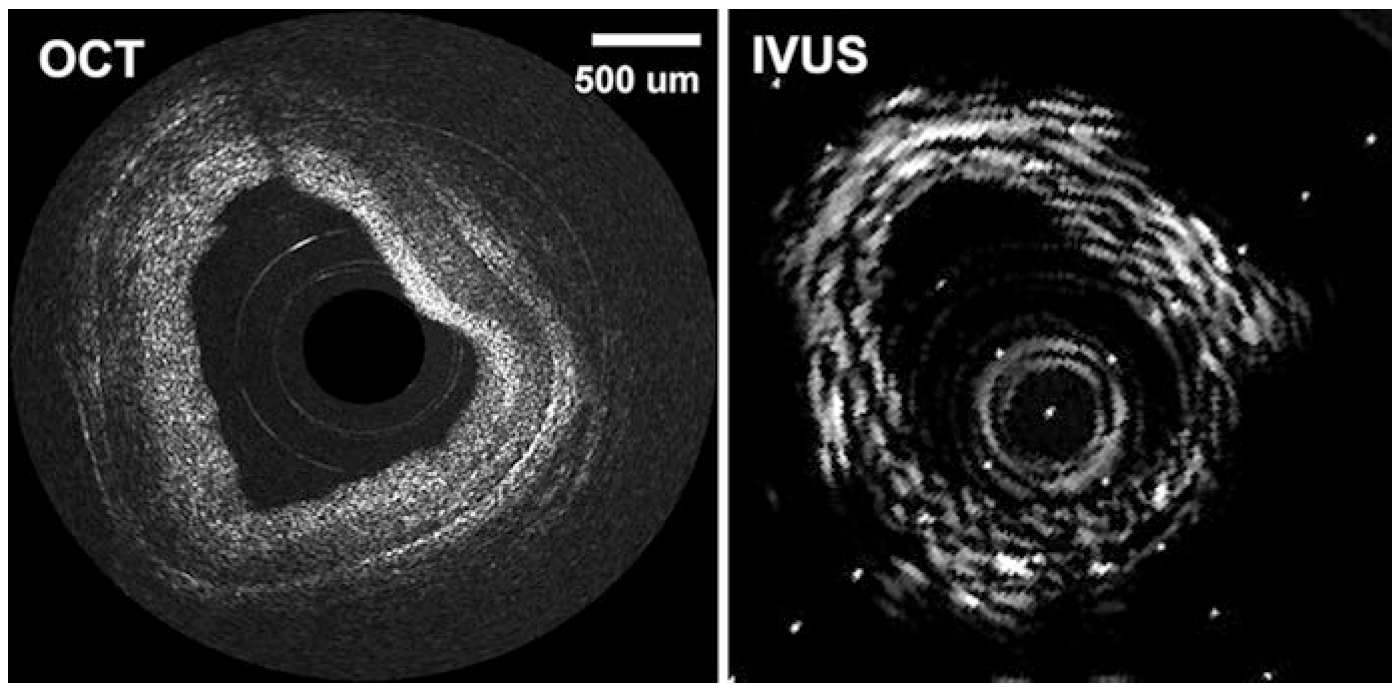
\includegraphics[width = \textwidth, keepaspectratio]{img/oct_intravascular_ultrasonido.png}
%	\caption[Comparación de OCT intravascular con ultrasonido]{Comparación de una imagen de OCT intravascular con ultrasonido (IVUS).}
%	\label{fig:oct_intravascular_ultrasonido}
%\end{figure}

%\subsubsection{Endoscopías y detección de cáncer con OCT}

%Por último, la OCT también ha sido empleada en el caso de la endoscopía. El primer estudio de endoscopía \invivo con imágenes de OCT fue realizado en 1997 \cite{Tearney1997, Sergeev1997}, un ejemplo de los resultados obtenidos por Tearney \emph{et al.} se muestra en la Fig.~\ref{fig:oct_endoscopia_conejo}. En la figura se observan las capas del esófago \emph{in vivo} de un conejo, en ella estructuras tales como la mucosa(m), submucosa(sm), mucosa interna (im), mucosa externa (om), serosa(s) y los tejidos de soporte vascular (a) pueden apreciarse. Los primeros estudios de endoscopía con imagen OCT en humanos fueron reportados por Sergeev \etal en 1997 \cite{Sergeev1997} y Feldchtein \etal en 1998 \cite{Feldchtein1998}, en donde se tomaron imágenes mediante  una sonda de barrido delantero en el canal de estándar. Estos estudios mostraron la utilidad de realizar OCT para imagen clínica de órganos tales como el esófago, la laringe, el estomago, la vejiga urinaria y el cuello uterino.


Por último, la OCT también ha sido empleada en el caso de la endoscopía. El primer estudio de endoscopía \invivo con imágenes de OCT fue realizado en 1997 \cite{Tearney1997, Sergeev1997}, en donde se obtuvieron los primeros resultados para el estudio del esófago de un conejo. Las imágenes de la OCT permitieron diferenciar de manera clara diferentes estructuras tales como la mucosa y la serosa. Los primeros estudios de endoscopía con imagen OCT en humanos fueron reportados por Sergeev \etal en 1997 \cite{Sergeev1997} y Feldchtein \etal en 1998 \cite{Feldchtein1998}, quienes mediante una sonda obtuvieron imágenes de membranas mucosas del esófago, la laringe, el estómago, la vejiga urinaria y el cuello uterino; mostrando así la utilidad de OCT en imagen clínica.

%\begin{figure}[ht!]
%	\centering
%	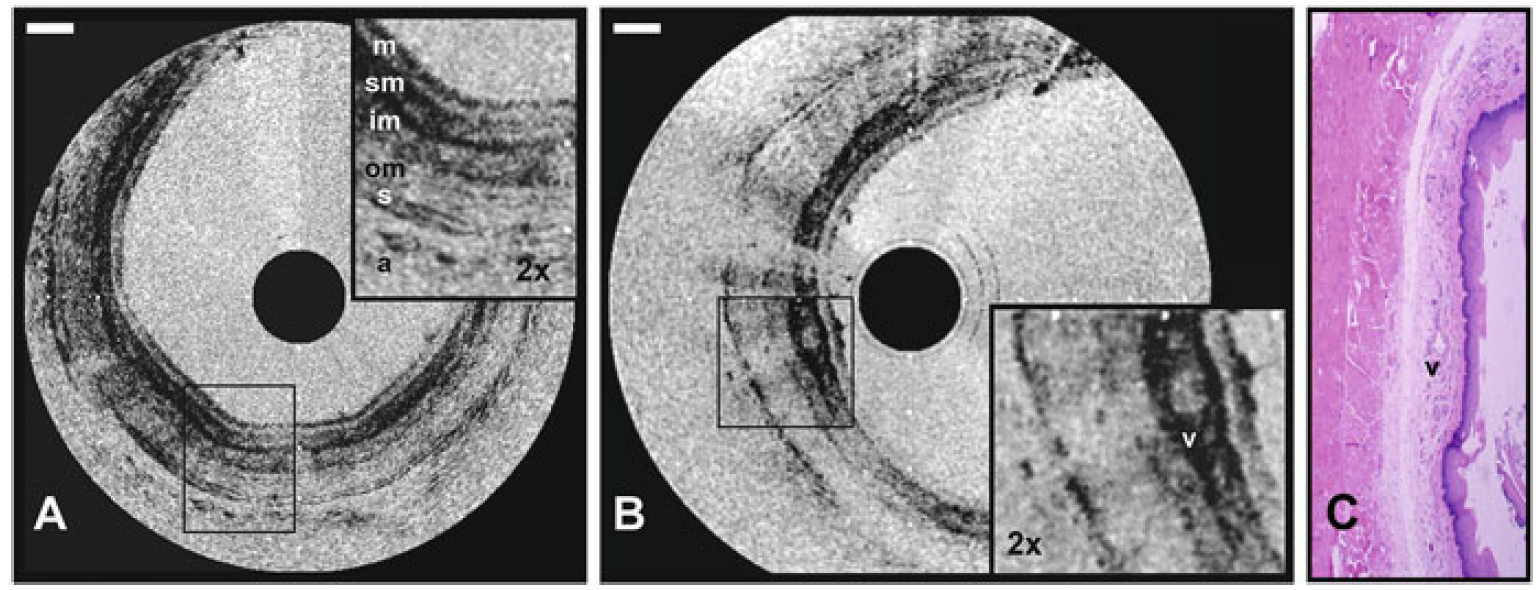
\includegraphics[width = \textwidth, keepaspectratio]{img/oct_endoscopia_conejo.png}
%	\caption[Endoscopía \emph{in vivo} del esófago de un conejo.]{Endoscopía \emph{in vivo} del esófago de un conejo. En la imagen (a) pueden observarse las capas del esófago, entre las que se aprecia: la mucosa(m), submucosa(sm), mucosa interna (im), mucosa externa (om), serosa(s) y los tejidos de soporte vascular (a). (v) es una vena que puede observarse en la submucosa. (c) histología. Escala $500um$. Tomada de Tearney \emph{et al.} \cite{Tearney1997}}
%	\label{fig:oct_endoscopia_conejo}
%\end{figure}

Dado el crecimiento de casos de cáncer en el esófago, estomago y colon, la endoscopía gastrointestinal tuvo una mayor atención, en contraste con esto, los estudios iniciales de OCT mostraron las ventajas de esta técnica para visualizar estructuras superficiales, ya que permite no solo ver las capas exteriores, sino que adicionalmente puede observar morfologías de tejidos bajo la superficie, permitiendo diferenciar patologías gastrointestinales, tales como el esógafo de Barret, los pólipos adenomatosos y el adenocarcinoma \cite{Bouma1999, Sergeev1997, Rollins1999, Jackle2000, Jackle2000_2, Sivak2000}. Los estudios de OCT para detección de cáncer son complejos, ya que los resultados de OCT deben ser comparados con técnicas estandarizadas tales como la biopsia que se ha convertido en un estándar en la detección de cáncer. El problema que tiene la OCT es que el contraste producido por las variaciones en las propiedades dispersivas de diferentes tejidos puede producir errores en las muestras tomadas dada la sensibilidad de OCT.

%\subsubsection{La tecnología del OCT en catéteres y endoscopios}

%El desarrollo de catéteres y endocopios ha sido fundamental para la implementación de OCT al interior del cuerpo \cite{Tearney1996, Tearney 1997_2}. La Fig.~\ref{fig:oct_cateter} muestra uno de los primeros sistemas de catéteres/endoscopios para OCT, el dispositivo posee una fibra óptica de modo único en un cable hueco rotatorio acoplado a una lente y a un microprisma que refleja la luz de radialmente. El haz es escaneado mediante la rotación del cable para generar una imagen transversa de la estructuras iluminadas. El diseño de este tipo de dispositivos para imagen mediante catéteres representa un desafío, ya que hay múltiples requerimiento tanto mecánicos, como ópticos y de biocompatibilidad que se deben abordar.

%\begin{figure}[ht!]
%	\centering
%	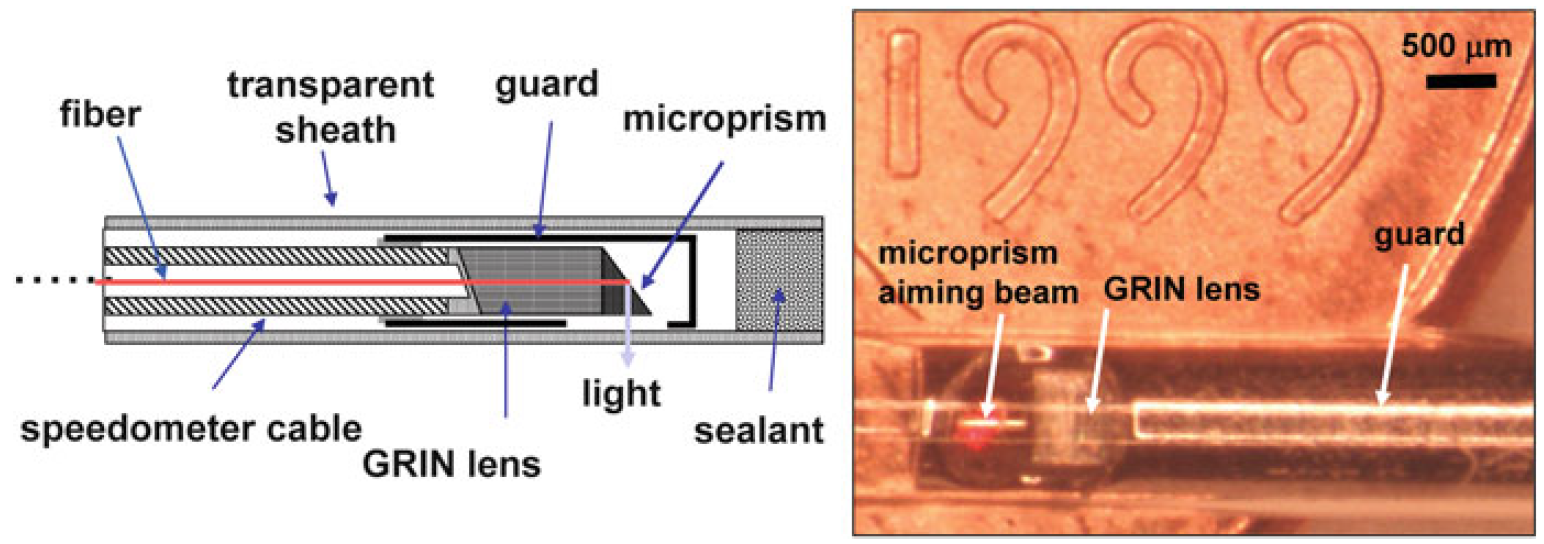
\includegraphics[width = \textwidth, keepaspectratio]{img/oct_cateter.png}
%	\caption[OCT mediante catéteres.]{Ejemplo de los primeros catéteres empleados para OCT.}
%	\label{fig:oct_cateter}
%\end{figure}

%
%Aunque OCT ha sido ampliamente estudiado y son constantes las nuevas publicaciones con propuestas, métodos, materiales y desarrollos, esta técnica aun presenta dificultades en su implementación. Un ejemplo de esto, es el escaneo lateral que debe realizarse para obtener las imágenes volumétricas
%
%La corrección del movimiento y la desviación producida por el escaneo son 
%
%El efecto que produce un muestro obliquo ha sido estudiado por 
%J. Walther, A. Krüger, M. Cuevas, and E. Koch. ``Effects of axial, transverse, and oblique sample motion in FD OCT in systems with global or rolling shutter line detector''. J. Opt. Soc. Am. A \textbf{25}(11), 2791-2802 (2008).
%
%
%
%
%Y han sido propiestas correcciones como
%M. Pircher, B. Baumann, E. Götzinger, H. Sattman, and C. Hitzenberger. ``Simultaneous SLO/OCT imaging of the human retina with axial eye motion correction''. Optics Express \textbf{15}(25), 16922-16932 (2007).
%
%S. Ricco, M. Chen, H. Ishikawa, G. Wollstein, J. Schuman, Correcting motion artifacts in retinal spectral domain optical coherence tomography via image registration. Med. Image Comput. Comput. Assist. Intervent. Miccai Proceedings \textbf{5761}, 100–107 (2009).
%
%B. Antony, M.D. Abramoff, L. Tang, W.D. Ramdas, J.R. Vingerling, N.M. Jansonius, K. Lee, Y.H. Kwon, M. Sonka, M.K. Garvin, Automated 3-D method for the correction of axial artifacts in spectral-domain optical coherence tomography images. Biomed. Opt. Exp. \textbf{2}, 2403–2416 (2011).
%
%
%
%Por otra parte, en OCT puede aparecer moteado (\textit{speckle}) causado por la dispersión que produce la muestra, aunque para OCT se han desarrollado algunos algoritmos de supresión de ruido, 

%Si bien OCT se ha expandido en la comunidad científica y médica, es de anotar que en el contexto científico Colombiano no se encuentra grupos de investigación vinculados a proyectos de desarrollo en áreas relacionadas con OCT. Por otra parte, las publicaciones internacionales por autores Colombianos que trabajen con OCT desde el punto de vista clínico también son escasas \cite{Hernandez2009,Homero2013}.

En general, dada la versatilidad y aplicabilidad de la OCT ha mostrado ser una técnica con altas posibilidades de implementación en diferentes áreas y aplicaciones de la medicina. Este documento presenta un marco teórico de los desarrollos y limitaciones que han surgido en la OCT con el fin de plantear un tema de investigación en esta área. Para dicho fin, el documento se encuentra organizado de la siguiente manera: en la Sección~\ref{sec:planteamiento_del_problema} se presenta el planteamiento del problema de investigación. En la Sección~\ref{sec:antecedentes_marco_teorico} se encuentran los antecedentes y marco teórico que detalla aspectos fundamentales a considerar sobre el desarrollo de la OCT. En la Sección~\ref{sec:objetivos} se presentará el objetivo general y los objetivos específicos que se espera completar con el trabajo de grado. La Sección~\ref{sec:metodologia} explicará en detalle los pasos propuestos para el desarrollo de las actividades y la realización de los objetivos específicos. La Sección~\ref{sec:cronograma} mostrará el cronograma planteado para el trabajo de grado, y posteriormente, se listarán los recursos necesarios para el desarrollo del trabajo de grado (Sección~\ref{sec:recursos}) y las referencias bibliográficas empleadas en este anteproyecto.

\section{Planteamiento del problema}
\label{sec:planteamiento_del_problema}

%En la implementación inicial de la OCT, conocida como OCT de primera generación o OCT en el dominio del tiempo [\textit{time-domain OCT}(TDOCT)], los datos en profundidad eran adquiridos mediante el desplazamiento axial del haz de referencia y posteriormente trasladando perpendicularmente el haz de escaneo. Sin embargo, hacia 1995 Fercher \etal \cite{Fercher1995} propusieron un nuevo método de medición cuyo funcionamiento era similar al de la OCT. La propuesta de Fercher consistía en medir el espectro de la luz, en lugar de tomar interferogramas a diferentes profundidades. El fundamento destrás de esta propuesta, es que el proceso de cambiar la distancia es equivalente a variar la longitud de onda, y se encuentran relacionados mediante una transformada de Fourier.



%En el sistema interferométrico sobre el cual se basa la OCT funciona a partir de una fuente blanca, haciendo uso del hecho de que la interferencia solo es producida en la región contenida dentro de la longitud de coherencia. Como se mencionó en la introducción, las imágenes volúmetricas son obtenidas en los siguientes pasos (Fig.~\ref{fig:scaningsystemoct}): primero se toman escaneos de manera axial para obtener el perfil de reflectividad en profundidad de la muestra, este proceso puede realizarse fácilmente a través del desplazamiento del espejo de referencia. Luego, se desplaza el haz objeto de manera lateral, es decir, en el plano $xy$ de la Fig.~\ref{fig:scaningsystemoct}. La interferencia es colectada por un foto detector, a continuación pasa por una etapa de adquisición de datos (DAQ) y finalmente los datos son transferidos hasta el computador.

%La Fig.~\ref{fig:scaningsystemoct} 

En la implementación inicial de la OCT, la información en profundidad es obtenida mediante desplazamientos axiales del haz de referencia que son producidos por actuadores tales como piezoeléctricos, así como lo indica la Fig.~\ref{fig:scaningsystemoct}. En ese sistema de OCT, la luz producida por la fuente viaja mediante una fibra óptica hasta llegar a un acoplador, en donde se divide por dos caminos diferentes; uno de ellos viaja directamente hasta el espejo de referencia que tiene la posibilidad de desplazarse en sentido axial. Posteriormente, el haz reflejado por el espejo regresa hacia la fibra óptica. El segundo haz es dirigido hacia un espejo de escaneo cuya función es desviar la luz que es proyectada en la muestra de manera controlada. Mediante este sistema, la porción de luz que sea reflejada por la muestra hacia la fibra óptica volverá a incorporarse al sistema óptico regresando hasta el acoplador. La información de los dos haces juntos llega entonces hasta un sensor que se encarga de obtener la señal interferométrica. El sensor transfiere los datos a un sistema de adquisición de datos (DAQ) y finalmente las señales son enviadas hasta el computador. 

La información volumétrica requiere que el haz proyectado hacia la muestra sea desplazado de manera lateral en dos direcciones, procedimiento que se ha realizado a través del uso de sistemas microelectromecánicos (MEMS) que permiten la inclinación controlada del haz, y por tanto el desplazamiento de éste sobre la muestra \cite{Zara2003,Jung2006,Aguirre2007}. El espejo de escaneo se encarga de mover el haz sobre el plano imagen produciendo imágenes bidimensionales de planos $xy$ a profundidades $z$ específicas, a este tipo de imagen se le conoce como \emph{en-face}. Una de las limitaciones de los sistemas para OCT surge justamente en la implementación del sistema de escaneo, ya que hay errores producidos no solo por la instrumentación sino por la misma muestra. 

\begin{figure}[th!]
	\centering
	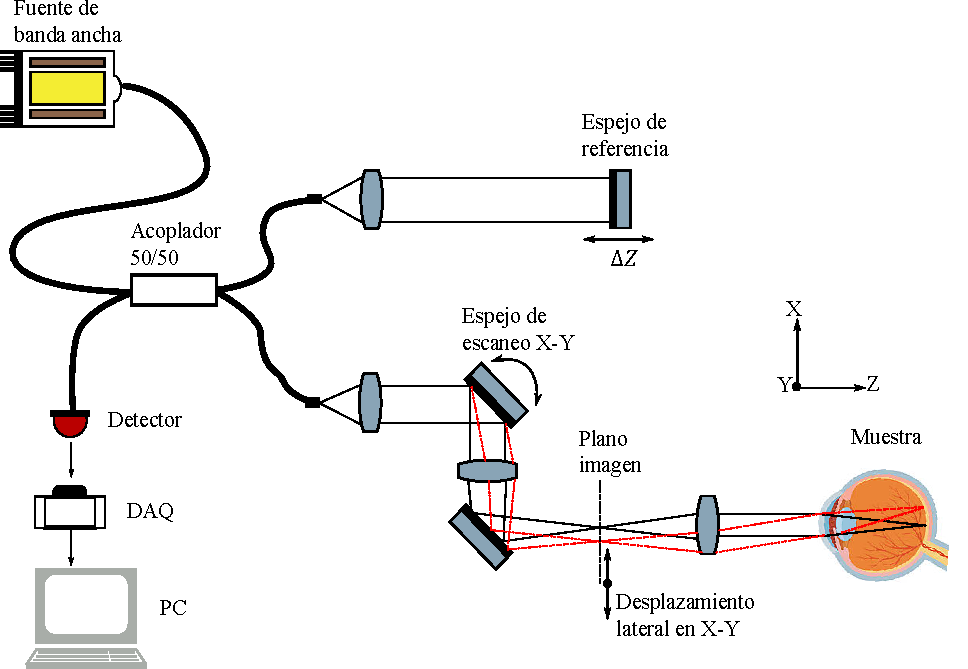
\includegraphics[width=0.7\linewidth]{img/scaning_system_oc.pdf}
	\caption{Sistema de escaneo para la OCT.}
	\label{fig:scaningsystemoct}
\end{figure}


Desde el punto de vista instrumental, algunos espejos de escaneo emplean sistemas de control retroalimentados tales como PID que se encargan del desplazamiento y control del sistema \cite{xie2004}, sin embargo, este tipo de control en lazo cerrado puede tener la falencia de enviar voltajes fluctuantes  que producen desviaciones, y pueden ser causados o bien por las constantes del controlador o por desplazamientos repentinos producidos por el paciente. Otros sistemas basados en MEMS \cite{Strathman2014} requieren voltajes AC para producir respuestas lineales, sin embargo, fluctuaciones en la frecuencia o en la amplitud del voltaje suministrado al actuador producen respuestas diferentes a la esperada. Adicionalmente, mientras se realizan los escaneos axiales, el espejo de escaneo se mueve a velocidad constante en las dos direcciones, por lo tanto hay una dirección con una velocidad menor (\emph{slow-axis}) y otro con una mayor velocidad (\emph{fast-axis}), esto hace necesario una corrección del movimiento en las imágenes de OCT obtenidas \cite{Yun2004, Pierce2005, Drexler2015}. En cuanto a la muestra que es tomada en pacientes, existen diferentes movimientos involuntarios que no pueden ser controlados, tales como la contracción muscular causada por la respiración o el parpadeo, así como cualquier movimiento que el paciente pudiera realizar mientras el sistema se encuentra en proceso de escaneo.

%Las limitaciones mencionadas anteriormente, si bien pueden no tener una incidencia directa sobre la reconstrucción de la reflectividad producida por la muestra, si tiene un impacto directo en la reconstrucción de la fase, a estos errores en la fase las denominaremos corrupciones de fase. Ahora bien, como se ha mencionado, la OCT se basa en la medición de la interferencia causada entre la luz dispersada por una muestra y un haz de referencia \cite{Huang1991}. Bajo este principio, la OCT es capaz de medir no solo la amplitud del campo reflejado por la muestra, sino que también puede medir su fase; tomando esto en cuenta, numerosas extensiones de OCT que emplean principalmente la fase han surgido bajo el nombre de \emph{phase resolved OCT}, entre estas sobresalen: OCT Doppler \cite{Chen1999}, microangiografía óptica \cite{Wang2010}, elastografía óptica de coherencia \cite{Ruikang2007} y OCT magnetomotriz \cite{Oldenburg2005}. En OCT Doppler por ejemplo, es común encontrar aplicaciones de flujometría, en el cual el sistema interferométrico de la OCT permite la detección de saltos en la fase causados por el movimiento de los centros dispersores en la muestra que no es posible observar con la amplitud. Mediante este proceso, es posible seguir el movimiento de los centros dispersores y cuantificar su velocidad de flujo \cite{Chen1999}. 

Ahora bien, como se ha mencionado, la OCT se basa en la medición de la interferencia causada entre la luz dispersada por una muestra y un haz de referencia \cite{Huang1991}. Bajo este principio, la OCT es capaz de medir no solo la amplitud del campo reflejado por la muestra, sino que también puede medir su fase. Los errores en la toma de datos que pueden ser producidos por el sistema de escaneo, así como el paciente, si bien pueden no tener una incidencia directa sobre la reconstrucción de la reflectividad producida por la muestra, si tiene un impacto directo en la reconstrucción de la fase; a estos errores en la fase los denominaremos corrupciones de fase. Numerosas extensiones de OCT que emplean principalmente la fase han surgido bajo el nombre de \emph{phase resolved OCT}, entre estas sobresalen: OCT Doppler \cite{Chen1999}, microangiografía óptica \cite{Wang2010}, elastografía óptica de coherencia \cite{Ruikang2007} y OCT magnetomotriz \cite{Oldenburg2005}. En OCT Doppler por ejemplo, es común encontrar aplicaciones de flujometría, en el cual el sistema interferométrico de la OCT permite la detección de saltos en la fase causados por el movimiento de los centros dispersores en la muestra que no es posible observar con la amplitud. Mediante este proceso, es posible seguir el movimiento de los centros dispersores y cuantificar su velocidad de flujo \cite{Chen1999}. 

Otro problema que es común en los datos adquiridos mediante OCT es el moteado (\textit{speckle}), el cual cumple una doble función ya que puede aportar información de la muestra o puede surgir como ruido \cite{Schmitt1999,Mariampillai2008}. En OCT el moteado como ruido surge cuando la señal que se registra en el detector posee información de la interferencia que se produce entre la luz dispersada por centros dispersores cercanos al área de escaneo, y en lugar de portar información sobre la muestra, degradan la calidad de la señal que se registra y dificultan su interpretación. En OCT existen diferentes técnicas de reducción de ruido multiplicativo \cite{Hughes2009,Szkulmowski2012,Aum2015}, aunque tienen la desventaja de poseer altos tiempos de procesamiento, y en algunos casos, requieren una imagen con bajo coeficiente señal-ruido para su correcto funcionamiento \cite{Fang2012}.

La propuesta para este trabajo de grado consiste en facilitar la interpretación y procesamiento de datos provenientes de OCT, mediante la implementación de técnicas de posprocesamiento que permitan mejorar la calidad de los datos adquiridos.